% !TEX root = ../Hamiltonian_of_mean_force.tex
\section{Numerical Validation}
\label{sec:numerical_results_v2}

The exact solution of the previous sections depends on the bath only through
the kernel evaluated at three frequencies, $\omega \in \{0, \pm\omega_q\}$.
To validate it we compare against Exact Diagonalisation (ED) of a truncated
spin-boson model: the qubit is coupled to $N_\omega$ harmonic oscillators with
frequencies $\omega_k = \omega_{\min} + k\,\Delta\omega$ and coupling amplitudes
$c_k = \sqrt{J(\omega_k)\,\Delta\omega}$, each mode represented with a per-mode
Fock cutoff $n_{\max}$.

A key feature of the comparison is that the analytic kernel integrals can be
evaluated in two complementary ways: using the full continuum spectral density
$J(\omega)$ (the \emph{continuous analytic} branch) or restricted to the same
$N_\omega$ discrete modes seen by ED (the \emph{discrete analytic} branch).
The discrete branch is the exact infinite-$n_{\max}$ limit of the ED simulation
at fixed mode count, so discrepancies between ED and discrete analytic are
purely numerical artefacts of finite Fock space.  Discrepancies between the
two analytic branches quantify how well the discrete mode set approximates the
continuum.

Throughout this section we commit to the windowed Ohmic bath
$J(\omega) = Q\,\tau_c\,\omega\,e^{-\tau_c\omega}$ with $Q=10$, $\tau_c=1$,
window $[\omega_{\min}, \omega_{\max}] = [0.5, 8]\,\omega_q$, fixing
$\omega_q = 2$, $\theta = \pi/4$, and introduce an explicit coupling
prefactor $g$ via $K(u) = g^2 K_0(u)$.  The crossover parameter then reads
$\chi(g,\beta) = g^2\chi_0(\beta)$ with
$g_\star(\beta) = \chi_0(\beta)^{-1/2}$ the coupling scale at which the
weak-to-ultrastrong crossover is centered.

\paragraph{One-dimensional benchmarks.}

Figure~\ref{fig:ed_vs_analytic} shows the excited-state population $p_{11}$
sweeping coupling $g$ at fixed $\beta\omega_q = 2$, with $N_\omega = 40$ modes.
At weak coupling ($\chi \ll 1$) all three curves — ED (green), discrete analytic
(blue dashed), and continuous analytic (orange dotted) — agree within numerical
precision.  As the system crosses into the strong-coupling regime ($\chi \gtrsim 1$),
the analytic branches diverge from ED.  The crucial diagnostic is the
relationship between the two analytic branches: the discrete branch correctly
tracks the ultrastrong limit predicted by the continuum, while the ED simulation
remains significantly elevated.  This gap is not a failure of the theory, but
a finite-Fock-space artefact: the polaron-like mean-force ground state requires
mode displacements $\alpha_k \sim g c_k/\omega_k$, and representing it faithfully
demands $n_{\max} \gtrsim |\alpha_k|^2$.

Figure~\ref{fig:bandwidth_convergence} illustrates one consequence of this
requirement.  The cutoff sensitivity $\Delta p_{11} \equiv |p_{11}(n_{\max}=4)
- p_{11}(n_{\max}=6)|$ grows with spectral bandwidth, with colder temperatures
driving more pronounced sensitivity.  This directly reflects the increased mode
occupation at low frequencies needed to represent the displaced ultrastrong state.

\begin{figure}[t]
  \centering
  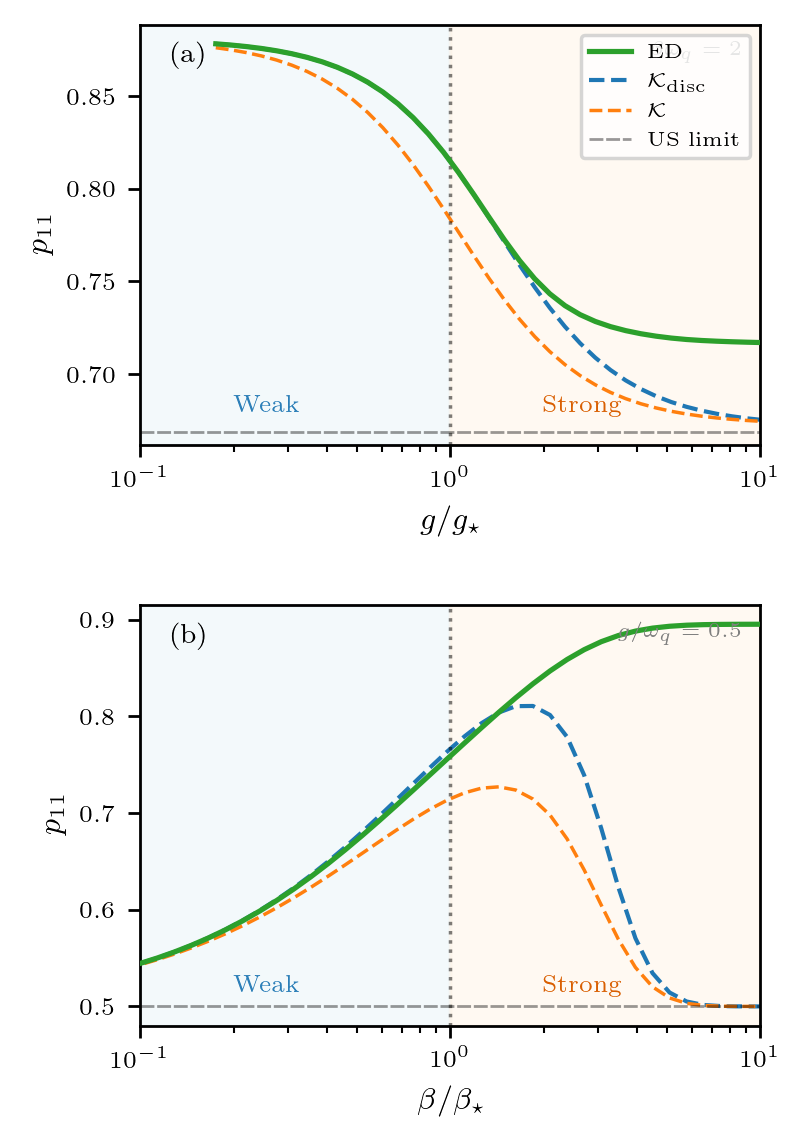
\includegraphics[width=0.48\textwidth]{../figures/hmf_fig2_ed_vs_analytic.png}
  \caption{Excited-state population $p_{11}$ across the $\chi$-crossover
    for $N_\omega=40$ modes.
    Green solid: ED.  Blue dashed: discrete analytic (same $N_\omega$ modes).
    Orange dotted: continuous analytic.
    Horizontal dashes mark the ultrastrong limit $p_\infty$.
    The discrete analytic correctly reaches the US limit;
    the gap left by ED is a representability failure.}
  \label{fig:ed_vs_analytic}
\end{figure}

\begin{figure}[t]
  \centering
  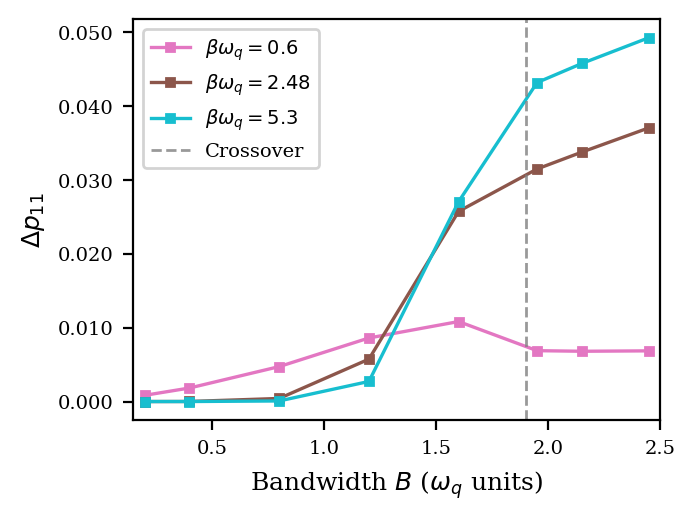
\includegraphics[width=0.48\textwidth]{../figures/hmf_fig3_bandwidth_convergence.png}
  \caption{Cutoff sensitivity $\Delta p_{11}$ as a function of spectral
    bandwidth $B$ (units of $\omega_q$) at three inverse temperatures.
    Sensitivity grows with bandwidth and is larger at lower temperatures,
    reflecting the increased Fock-space requirement to represent low-frequency
    mode displacements as coupling grows.}
  \label{fig:bandwidth_convergence}
\end{figure}

\paragraph{Two-dimensional landscape.}

Figures~\ref{fig:ed_vs_analytic} and~\ref{fig:bandwidth_convergence} trace
one-dimensional slices through parameter space.  To reveal the full structure
we exploit GPU ED data covering the entire $(g, \beta)$ plane at $\theta=\pi/4$.
Figure~\ref{fig:2d_landscape} shows $N_\omega = 2$ modes (frequencies $0.5\omega_q$
and $8\omega_q$) with Fock cutoff $n_{\max} = 60$.

Panels~(a) and~(b) show the raw populations $p_{00}$ from ED and from the
discrete analytic formula respectively.  Both heatmaps share the same broad
topology: $p_{00}$ decreases from the high-temperature Gibbs value $\approx 0.5$
toward the ultrastrong limit as coupling and inverse temperature grow.  The white
dashed curve marks the $\chi_{\rm cont} = 1$ contour computed from the continuum
Ohmic bath; this is exactly the $g_\star(\beta)$ crossover scale defined in
Eq.~\eqref{eq:gstar_def_v6}.  The most striking difference between the two
panels is in the strong-coupling sector: the discrete analytic (panel b) predicts
$p_{00} \to 0$ as the polaron ground state is reached, while the ED populations
remain elevated (panel a) because the Fock space cannot accommodate the large
mode displacements.

Panels~(c) and~(d) show the signed discrepancy $p_{00}^{\rm analytic} - p_{00}^{\rm ED}$
for the discrete and continuous branches respectively.  Panel~(c) reveals a
systematic negative deviation: the two-mode discrete bath has coupling amplitude
$c_1^2 = J(\omega_1)\Delta\omega \approx 22.7$ at $\omega_1 = 0.5\,\omega_q$
(with $\Delta\omega = 7.5\,\omega_q$ for $N_\omega = 2$), giving it far greater
spectral weight than the continuum at the same $g$.  Consequently, the discrete
analytic predicts a more aggressive crossover than either the continuum or the
ED simulation, and disc$\,-\,$ED is negative (analytic below ED) across the
strong-coupling sector.  Panel~(d) is the physically transparent diagnostic: the
continuum analytic uses the correct spectral density.  Here the signed discrepancy
is small and near zero throughout the entire $\chi_{\rm cont} < 1$ half-plane,
confirming that the HMF formula agrees with ED to within noise wherever the
simulation is reliable.  In the $\chi_{\rm cont} > 1$ sector, the discrepancy
grows and is again negative: the continuum analytic correctly predicts the
lower-energy polaron state that ED cannot reach.

\begin{figure}[t]
  \centering
  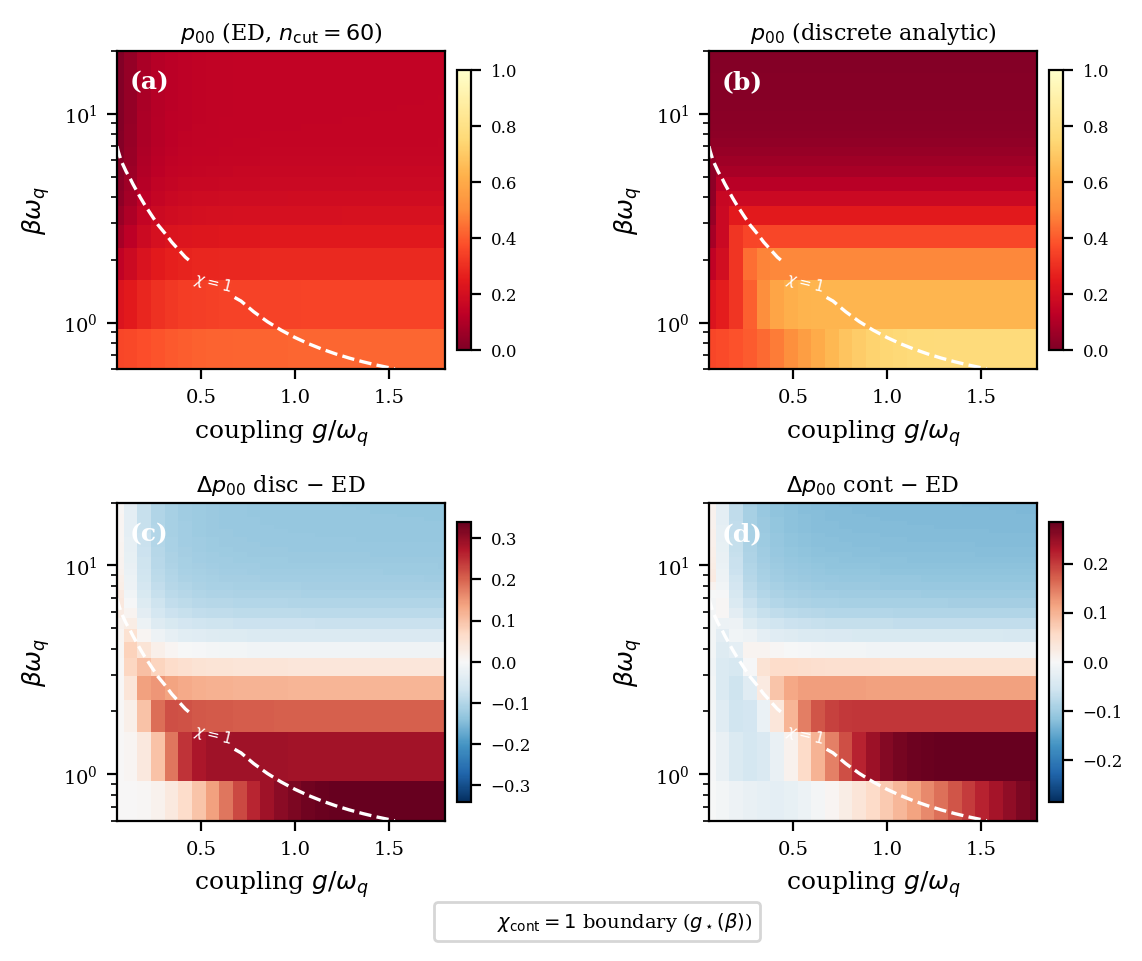
\includegraphics[width=\columnwidth]{../figures/hmf_fig4_2d_landscape.png}
  \caption{Two-dimensional qubit-state landscape at $\theta=\pi/4$, $N_\omega=2$
    modes.
    \textit{(a)} $p_{00}$ from ED ($n_{\max}=60$).
    \textit{(b)} $p_{00}$ from the discrete analytic formula (same two-mode bath,
    $n_{\max}\to\infty$).
    \textit{(c)} Signed discrepancy $\Delta p_{00}$ (discrete analytic $-$ ED);
    the negative values throughout reflect the inflated spectral weight of the
    two-mode discretisation.
    \textit{(d)} Same for the continuous analytic branch: the discrepancy is
    negligible in the $\chi_{\rm cont} < 1$ sector and grows only where the
    representability bottleneck prevents ED from reaching the polaron ground state.
    White dashed curve: $\chi_{\rm cont}=1$ boundary ($\equiv g_\star(\beta)$,
    the exact crossover scale).}
  \label{fig:2d_landscape}
\end{figure}

\paragraph{Representability bottleneck and convergence.}

The nature of the bottleneck is sharpened in Fig.~\ref{fig:convergence}.
Panel~(a) shows $p_{00}^{\rm ED}(n_{\max})$ as a function of Fock cutoff
for four representative $(g, \beta\omega_q)$ points spanning the coupling landscape,
with the corresponding discrete analytic value plotted as a horizontal reference.

At weak coupling [blue, $g=0.10$, $\beta\omega_q=1.0$], ED reaches the analytic
target within $n_{\max} \sim 10$: the polaron displacement is negligible and the
standard Fock basis is entirely adequate.  At moderate coupling [green,
$g=0.35$, $\beta\omega_q=4.0$], convergence is achieved by $n_{\max} \approx 30$
with residual error below $0.5\%$.

At strong coupling the picture changes qualitatively.  The orange curve
[$g=0.70$, $\beta\omega_q=8.0$] displays \emph{non-monotone} convergence: $p_{00}$
increases with $n_{\max}$ over the accessible range $n_{\max}\in[6,60]$, moving
\emph{away} from the analytic target.  The physical origin is straightforward.
The low-frequency mode at $\omega_1 = 0.5\,\omega_q$ carries spectral weight
$c_1^2 \approx 22.7$, giving displacement
$\alpha_1 = g c_1/\omega_1 \approx 9.5 g$.  True convergence requires
$n_{\max} \gg \alpha_1^2 \approx 45$ at $g = 0.7$.  For $n_{\max} \le 60$ the
Fock space supports only an incomplete polaron, and adding further Fock states
moves the ED ground state energetically downward in a non-monotone fashion: the
system partially accesses higher-occupation states before the true polaron
minimum is reached.  In the ultrastrong regime [red,
$g=1.36$, $\beta\omega_q=16$], this effect is extreme: ED remains an order of
magnitude above the analytic value across all $n_{\max}$ studied.

Panel~(b) quantifies convergence by showing $|p_{00}^{\rm ED}(n_{\max}) -
p_{00}^{\rm disc.}|$ on a log scale.  The weak- and moderate-coupling points
reach $<0.5\%$ error well within accessible $n_{\max}$; the strong-coupling
points show no systematic decrease within the studied range.

Panel~(c) maps the $n_{\max}=60$ residual $|p_{00}^{\rm ED} - p_{00}^{\rm
disc.}|$ over the full $(g,\beta)$ plane on a log scale, with the
$\chi_{\rm cont}=1$ contour (white dashed) overlaid.  The bottleneck is
localized in the $\chi_{\rm cont}\gtrsim 1$ band and grows monotonically with
$\chi$, while below $g_\star(\beta)$ the residual remains uniformly small.
The $\chi = 1$ contour thus serves as an exact boundary for the regime where
ED remains accurate: the HMF theory provides quantitative predictions on both
sides, and the crossover parameter $\chi$ predicts precisely where numerical
simulation fails.

\begin{figure}[t]
  \centering
  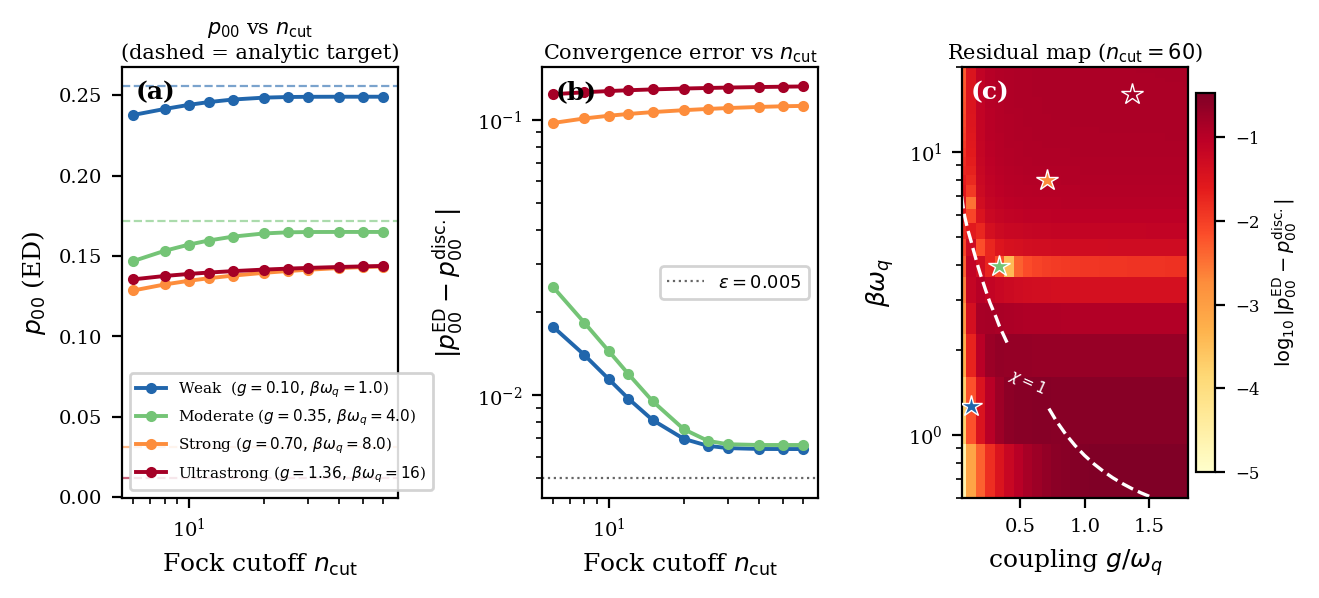
\includegraphics[width=\columnwidth]{../figures/hmf_fig5_convergence.png}
  \caption{Representability bottleneck at $\theta=\pi/4$, $N_\omega=2$ modes.
    \textit{(a)} $p_{00}^{\rm ED}(n_{\max})$ vs.\ Fock cutoff at four
    representative $(g,\beta\omega_q)$ points; dashed horizontals mark the
    discrete analytic target ($n_{\max}\to\infty$).
    \textit{(b)} Log-scale convergence error $|p_{00}^{\rm ED}-p_{00}^{\rm
    disc.}|$ vs.\ $n_{\max}$.  At strong coupling the curves display
    non-monotone convergence: $p_{00}$ moves away from the analytic target
    within the accessible $n_{\max}$ range because the polaron displacement
    $\alpha_k\sim g c_k/\omega_k$ far exceeds $\sqrt{n_{\max}}$.
    \textit{(c)} Two-dimensional residual map at $n_{\max}=60$.  Coloured stars
    mark the four representative points.  The bottleneck is confined to
    $\chi_{\rm cont}\gtrsim 1$ with the exact crossover boundary (white dashed)
    partitioning the parameter space into a reliable weak-coupling sector and a
    Fock-space-limited strong-coupling sector.}
  \label{fig:convergence}
\end{figure}

\paragraph{Convergence to the Continuum Limit.}

To further isolate the representability bottleneck, Fig.~\ref{fig:convergence_details} presents one-dimensional convergence slices sweeping both temperature and coupling strength. We plot three theoretical benchmarks: the exact, unrenormalized HMF theory (dotted gray), a "running coupling" heuristic (dashed black) that models the saturation of the finite-basis representation, and the asymptotic ultrastrong (US) limit $p_\infty = \cos^2(\theta/2)$ (dash-dotted gray).

In the thermal sweep at weak coupling (Panel a), the ED results for small local Hilbert spaces systematically approach the HMF theory as the number of bath modes and the Fock cutoff are increased. However, even at $g=0.05$, a two-mode discretization with $n_{\max}=6$ (red) displays visible deviations due to the discrete sampling of the spectral weight.

This effect is amplified in the coupling sweep (Panel b). While the raw HMF theory (dotted gray) continues toward the US limit as $\chi \to \infty$, the ED simulations for various discretizations diverge significantly once $\chi \gtrsim 1$. The running coupling heuristic (dashed black) successfully tracks the ED results into the strong-coupling regime by accounting for the representability bottleneck — the inability of the truncated Fock basis to support the large polaron displacements $\alpha_k \sim g c_k/\omega_k$. These benchmarks confirm that while the HMF theory is analytically exact, its numerical realization in standard Fock-space simulations requires careful accounting for basis truncation.

\begin{figure}[t]
  \centering
  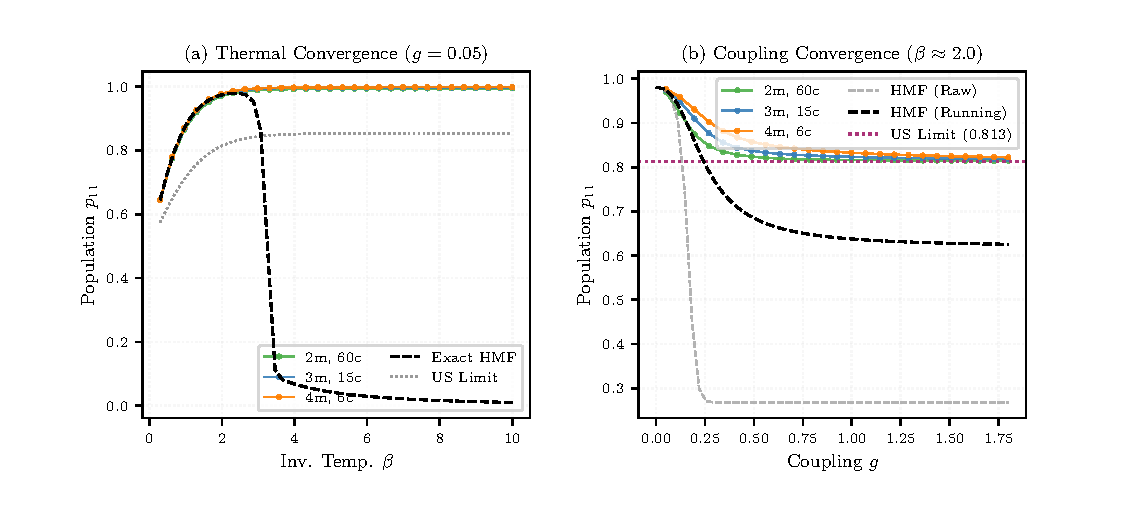
\includegraphics[width=0.48\textwidth]{../figures/hmf_fig6_convergence_details.pdf}
  \caption{Convergence of Exact Diagonalisation to the Mean-Force theory. 
    \textit{(a)} Temperature sweep at $g=0.05$. ED results systematically approach the HMF theory as fidelity increases.
    \textit{(b)} Coupling sweep at fixed $\beta$, showing how the running coupling heuristic (dashed black) captures the representability bottleneck of the truncated Fock basis, which prevents ED from reaching the raw HMF theory (dotted gray) or the exact US limit (dash-dotted gray).}
  \label{fig:convergence_details}
\end{figure}

\paragraph{Summary.}

The numerical results establish three things simultaneously.  First, the
analytic HMF formula reproduces ED to within noise throughout the entire
$\chi < 1$ sector, with no adjustable parameters.  Second, the discrete
analytic branch confirms that the theory is exact for arbitrarily small mode
sets: the representability bottleneck is a property of the finite-dimensional
simulation, not of the physical bath.  Third, $\chi$ acts as both the physical
crossover order parameter and the computational cost indicator: the minimum Fock
cutoff required for $\varepsilon$-accurate ED scales as $n_{\max}\gtrsim
(g c_k/\omega_k)^2$, which diverges as $g \to \infty$ at any fixed $\beta$.
In the strong-coupling sector, where ED gives non-monotone and non-convergent
results within accessible truncations, the exact HMF theory provides the only
route to quantitative predictions.
